\documentclass{sig-alternate}
\usepackage{times}
\usepackage{amssymb,amsmath}
\usepackage{cleveref}
\usepackage{algorithm}
\usepackage{times}
\usepackage{color}
\usepackage{url}
\usepackage{subfigure}
\usepackage{xspace}
\usepackage[noend]{algorithmic}
\usepackage{enumerate}
\usepackage{multirow}
\usepackage{balance} 
\usepackage{epstopdf}
\usepackage{graphicx}

\newcommand{\model}{{{\sf SourceNote}}\xspace}
\newtheorem{definition}{Definition}
\newtheorem{example}{Example}
\newtheorem{theorem}{Theorem}
\newtheorem{problem}{Problem}
\newtheorem{reduction}{Reduction}


\begin{document}

\conferenceinfo{7th Biennial Conference on Innovative Data Systems Research (CIDR`15)}{January 4-7, 2015, Asilomar, California, USA.}

%\title{Assessing the Quality of Data and Finding Invaluable Sources}
%\title{Finding Quality in Volume: The Challenge of Discovering Valuable Sources for Integration}
\title{Finding Quality in Quantity: The Challenge of Discovering Valuable Sources for Integration}
%\title{SourceNote: Discovering Invaluable Data Sources in Volume}

\numberofauthors{5} 

\author{
% 1st. author
\alignauthor
Theodoros Rekatsinas\\
       \affaddr{University of Maryland}\\
       \email{thodrek@cs.umd.edu}
% 2nd. author
%\alignauthor
%Amol Deshpande\\
%       \affaddr{University of Maryland}\\
%       \email{amol@cs.umd.edu}
% 3rd. author
\alignauthor
Xin Luna Dong\\
       \affaddr{Google Inc.}\\
       \email{lunadong@google.com}
 \and
% 4th. author
\alignauthor
Lise Getoor\\
       \affaddr{UC Santa Cruz}\\
       \email{getoor@soe.ucsc.edu}
 % 5th. author
\alignauthor
Divesh Srivastava\\
       \affaddr{AT\&T Labs-Research}\\
       \email{divesh@research.att.com}
}    

\maketitle
\begin{abstract}
Data is becoming a commodity of tremendous value for many domains. This is leading to a rapid increase in the number of data sources and public access data services, such as cloud-based data markets and data portals, that facilitate the collection, publishing and trading of data. Data sources typically exhibit wide variety and heterogeneity in the types or schemas of the data they provide, their quality, and the fees they charge for accessing their data. Users who want to build upon such publicly available data, must (i) identify sources that are relevant to their applications, (ii) discover sources that collectively satisfy the quality and budget requirements of their applications, with few effective clues about the quality of the sources, and (iii) repeatedly invest many person-hours in assessing the eventual usefulness of data sources. All three steps require investigating the content of sources manually,  integrating them and evaluating the actual benefit of the integration result for a desired application. Unfortunately, when the number of data sources is large, humans have a limited capability of reasoning about the actual quality of sources and the trade-offs between the benefits and costs of acquiring and integrating sources. In this paper we explore the problems of automatically appraising the quality of data sources and identifying the most valuable sources for diverse applications. We introduce our vision for a new {\em data source management system} that automatically assesses the quality of data sources based on a collection of rigorous data quality metrics and enables the automated and interactive discovery of valuable sources for user applications. We argue that the proposed system can dramatically simplify the {\em Discover-Appraise-Evaluate} interaction loop that many users follow today to discover sources for their applications. 
\end{abstract}

% A category with the (minimum) three required fields
%\category{H.4}{Information Systems Applications}{Miscellaneous}
%A category including the fourth, optional field follows...
%\category{D.2.8}{Software Engineering}{Metrics}[complexity measures, performance measures]

%\terms{Theory}

%\keywords{ACM proceedings, \LaTeX, text tagging} % NOT required for Proceedings

\section{Introduction}
In the last few years, the number of data sources available for integration and analysis has increased many-fold because of the ease of publishing data on the Web, the proliferation of services that facilitate the collection and sharing of data (e.g., Google Fusion Tables), and  the adoption of open data access policies both in science and government. This deluge of data has enabled small and medium enterprises as well as data scientists and analysts (e.g., political or business analysts) to acquire and integrate data from multiple data sources. Although much of the data is freely available, the number of data sources that charge monetary costs for access is rapidly increasing, a trend that is expected to continue as data is further commoditized~\cite{balazinska:vldb11}. 

Given the high number of available data sources and the fact that acquiring data may involve a monetary cost, it is challenging for a user to identify sources that are truly beneficial to her application. In fact, sources may provide erroneous or stale data~\cite{Dong_vldb:2009, li:2012}, they may provide duplicate data at different prices, and may exhibit significant heterogeneity in the representation of stored data, both at the schema and the instance level~\cite{bronzi:2013, li:2012, dassarma:2012}. After choosing a set of sources to use, a substantial effort must be spent in cleaning the sources, extracting structured information from them (for unstructured sources), constructing schema mappings, resolving entity references, and setting up the overall integration pipeline for continuous ingest; hence the initial selection of sources becomes even more important. The above give rise to the natural question of how can one discover {\em valuable sources}, i.e., sources that maximize the user's benefit at the minimum cost. Recent work~\cite{dong:vldb13,rekatsinas:2014} showed how, given a fixed data domain, the benefit of integration can be quantified using rigorous data quality metrics, such as {\em coverage}, {\em accuracy} and {\em freshness}, and introduced the paradigm of {\em source selection} to reason about the benefits and costs of acquiring and integrating data from static and dynamic sources. This line of work showed how one can identify the set of sources that can maximize the marginal gain for a predefined benefit function using a fixed quality metric or a fixed weighting scheme across different quality metrics. However, the proposed techniques are not sufficient for general users. 

First, the data quality metrics used to quantify the benefit of integration are complex and it is not easy, especially for general users, to understand the trade-offs between these metrics. Having a fixed and predefined weighting mechanism among different quality metrics does not allow the user to understand the implications of the quality trade-offs for source selection and identify the set of sources that truly fits her requirements. We illustrate this using the following example inspired by recent work by Schutte et al.~\cite{schutte:2014}.
\vspace{-5pt}
\begin{example}
Consider a political scientist who wants to find data providing supporting evidence for a new theory on causal relationships between interactions among different actors (including individuals, international organizations or countries) at a specific location. Such interactions are usually reported in newspapers, thus, our system should allow the political scientist to discover the newspapers whose news articles will provide her with sufficient data either supporting or contradicting her theory. The completeness (i.e., coverage) and accuracy of data are important here but the freshness of data is not crucial as delayed mentions of actor interactions will not affect the evidence provided by the data. While this distinction between coverage and freshness is clear, i.e., the scientist may require that freshness is completely ignored, the correct trade-off between accuracy and coverage is not well known in advance. In fact demanding only highly accurate data may limit the coverage of events significantly, thus, the user should have the flexibility to explore and understand the trade-off between accuracy and coverage. 
\end{example}
Second, the existing source selection techniques do not allow the user to evaluate the result returned by the system. The current techniques focus on finding a single set of sources that maximizes the marginal gain between the benefit and cost of integration given a budget constraint by the user, and report the overall quality and cost characteristics to the user. This does not allow the user to understand the individual quality and cost contribution of each selected source to the final result. Providing this information and enabling the user to {\em interactively explore} how the source selection solution will be affected by adding or removing sources is necessary to evaluate the solutions returned by the source management system. Finally, previous techniques focus on fixed domains and do not support source selection for arbitrary applications in multi-user environments with diverse tasks.  

In this paper, we introduce our vision for a {\em data source management system} that enables users to discover the most valuable data sources for their applications. We present how such a system can support the interactive exploration of different sets of sources, allowing the user to truly understand the quality and cost trade-off between different integration options. To enable the latter, we show how one can extend traditional knowledge bases with a {\em correspondence graph} to reason about the content and quality of data sources. We also extend the paradigm of source selection to a multi-objective optimization problem that allows users to make optimal decisions in the presence of trade-offs between conflicting objectives (e.g., different data quality or budget requirements).

The remainder of the paper is organized as follows. In \Cref{sec:overview} we provide an overview of the architecture of a data source management system, the key functionalities it should support and discuss the main challenges in building such a system. In \Cref{sec:corgraph} we present our proposed data source management system, introduce the different modules of the system and propose techniques for addressing the aforementioned challenges. Finally, \Cref{sec:related} discusses related work and \Cref{sec:conclusion} concludes the paper. 

\section{Data Source Management}
\label{sec:overview}
In this section we provide an overview of our proposed data source management system, and discuss the key functionalities such a system needs to support. Furthermore, we present the key challenges in each of these functionalities.

\subsection{System Overview}
\label{sec:architecture}
We envision a data source management system following the architecture shown in \Cref{fig:system}. The system is composed of (i) a data extraction module, (ii) a source analysis engine and (iii) a query engine. The basic operations of a data source management system can be divided into an {\em offline} phase and an {\em online} phase. During the offline phase, the data extraction module is responsible for extracting and storing raw data from different data sources. Then, the source analysis engine analyzes this raw data to identify the content of sources, evaluates their quality with respect to a collection of data quality metrics and constructs an index describing both the content and the quality of each source. This index will be used during the online phase when a user interacts with the system and discovers the most valuable sources for her application. The aforementioned operations may be performed once, if the sources are static, or repeatedly over time, if the sources are dynamic and their content changes. 
\begin{figure}
	\begin{center}
	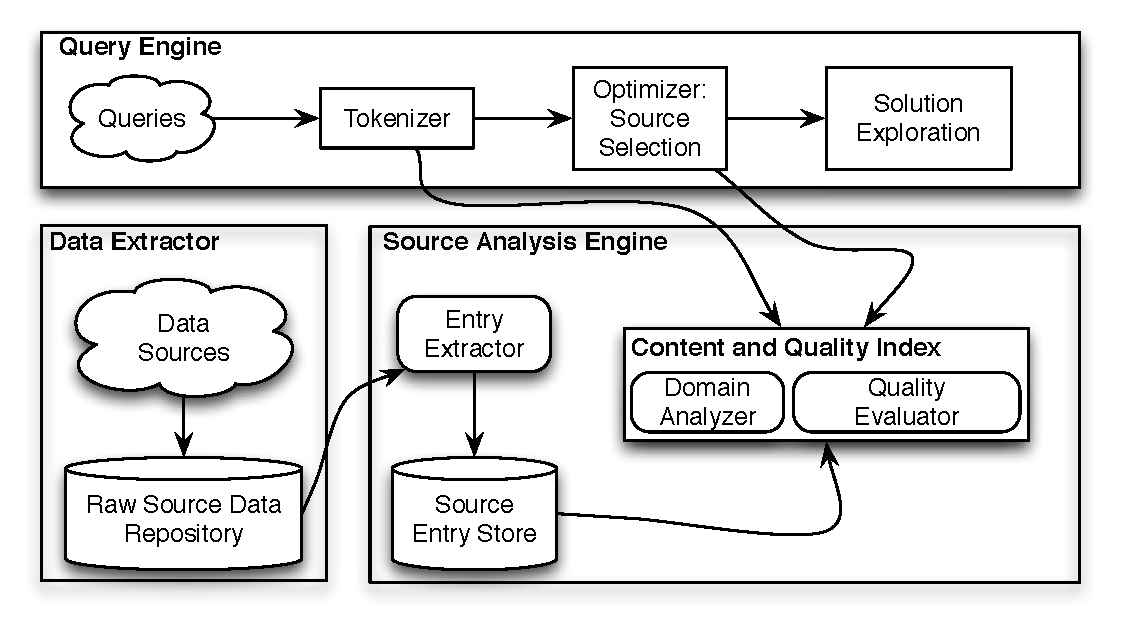
\includegraphics[clip,scale=0.5]{fig/system.eps}
	\vspace{-20pt}
	\caption{Source Management System Architecture.}
	\label{fig:system}
	\end{center}
	\vspace{-20pt}
\end{figure}
During the online phase, a user gives a description of her requirements as input to the query engine which detects the most valuable sources using source selection. Typically a user would start by providing the following information: (i) a free-text description of the task corresponding to a collection of mentions to either abstract concepts (e.g., ``commerce treaties'') or specific objects, such as locations, organizations, people and items, (ii) a selection of relevant data quality metrics from a list of supported metrics, and (iii) a desired budget characterizing the amount of money the user can afford for acquiring data. Given these specifications as input, the query engine should perform the following operations:
\begin{enumerate}
\item {\bf Discover.} The system should automatically determine which sources are relevant to the task by mapping the content of the task description to the content of sources.
\item {\bf Appraise.} After discovering the relevant sources, the system should automatically find subsets of sources that, if integrated together, maximize the integration quality under the budget requirements of the user. If available, the system should identify multiple solutions that correspond to different trade-offs among different quality metrics. 
\item {\bf Evaluate.} The solutions discovered in the previous phase should be presented to the user together with a concise description of their quality characteristics as well as a description of the data sources included in each of them. Moreover, the user should be able to interactively explore the returned solutions either by removing sources from a recommended solution or by examining solutions with similar characteristics that contain different sources. The latter enables the user to identify the solution that is best suited for her task.
\end{enumerate}

\subsection{Challenges}
We now discuss the main challenges in each of the operations presented above. 
\subsubsection{Analyzing the Content of Sources}
\label{sec:content}
The first challenge is analyzing the content of diverse data sources and being able to identify the data domain of each source. This is necessary for a multi-user environment where users with varying requirements interact with the system. For example, the data source management system should be able to analyze the content of a structured Web table providing financial data and the unstructured content of news articles extracted from a newspaper. Therefore, a data source management system should be able to reason about the semantic content of different types of data ranging from tables to DOM trees to free-text. To do this, the proposed system needs to analyze the content of all available sources. Accessing the entire content may not be possible for all sources as many require a monetary fee for accessing their data. Nevertheless, there are many cases where sources offer free samples or limited-transaction access to their content. This raises further challenges, such as how can one obtain a comprehensive view on the different concepts covered by a data source, how often should one obtain and analyze content samples to identify the rate of change for a source and how can one determine the right samples to obtain an accurate estimate of the source's quality.

\subsubsection{Data Source Quality Metrics} 
\label{sec:quality}
The second challenge is defining the quality of data. Measuring the quality of a data source requires reasoning about the content of the source with respect to some specific {\em context}. For example, ``ESPN'' is a high coverage source for ``sports in the USA'' but has zero coverage for politics. To formalize the notion of context we introduce the concept of a {\em data cluster}. A data cluster corresponds roughly to a set of concepts and concept instances (e.g., specific sports, countries, organizations) defining a specific data domain (e.,g Sports in the USA). \textcolor{red}{A formal definition of a data cluster is presented in \Cref{sec:corgraph}. To measure the quality of a data source with respect to a cluster, one needs to compare the data provided by the source to the real-world objects contained in that cluster. These real-world objects correspond to elemental data entries associated with any of the {\em concept instances} (e.g., Baseball in the USA) contained in the data cluster. A source may provide data entries from multiple clusters, and thus, it can have multiple quality profiles corresponding to different clusters.}

Traditionally, the quality of data sources had been measured using the percentage of data and the amount of erroneous information provided by the source. In the last decade, however, there has been a growing interest in defining diverse metrics to assess the quality of data~\cite{pipino:2002}. Nevertheless, most of these metrics are hard to quantify and measure for arbitrary datasets. Next, we focus on a collection of data quality metrics that can be expressed as probability distributions and hence admit rigorous definitions. The following list extends metrics introduced in our recent work~\cite{dong:vldb13, rekatsinas:2014}.

\textcolor{red}{Let $\mathcal{C}$  be a data cluster,  $\mathcal{C}.I$ be the set of concept instances corresponding to $\mathcal{C}$ and $\mathcal{C}.D$ be the set of all real-world objects (i.e., elemental data entries) that are relevant to $\mathcal{C}$. Moreover, let $\mathcal{C}[i].D$ be the set of all data entries that are associated with a concept instance $i \in \mathcal{C}.I$. Notice, that $\mathcal{C}.D$ is not fully known but only partial information is available for the content of this cluster via the data sources. We assume that each object $e \in \mathcal{C}.D$ has a set of attribute values denoted by $e.A$. For example, these attributes may correspond to a location or an organization or a time point. Moreover, we assume that both the objects in $\mathcal{C}.D$ and their values may change over time. Given a set of sources $\bar{S}$ relevant to cluster $\mathcal{C}$ and an integration model $F$ we have $F_C(\bar{S}) \subseteq \mathcal{C}.D$, where $F_C(\bar{S})$ denotes the set of data entries extracted after integrating all sources in $\bar{S}$ that are related to $\mathcal{C}$. Similarly $F_C(\bar{S})[i]$ corresponds to the entries in $F_C(\bar{S})$ relevant to instance $i \in \mathcal{C}.I$. Using this notation we define the following metrics:}

\textcolor{red}{\vspace{3pt}\noindent\textbf{Coverage.} The coverage of $\bar{S}$ with respect to $\mathcal{C}$ can be defined as a multinomial distribution over all elemetns of $\mathcal{C}.I$ where the probability value for each instance $i \in \mathcal{C}.I$ corresponds to the probability that a data entry $e$ chosen from $\mathcal{C}[i].D$ uniformly at random will be present in $F_C(\bar{S})$. Notice that we do not require that the attributes of the object $e.A$ are correct. One can easily generalize this definition to a cluster-based coverage measure corresponding to a single probability value considering all the entries contained in $\mathcal{C}.D$.}

\textcolor{red}{\vspace{3pt}\noindent\textbf{Accuracy.} The accuracy of $\bar{S}$ with respect to $\mathcal{C}$ can be defined as a multinomial distribution over all instances of $\mathcal{C}.I$ where the probability value for an element $i \in \mathcal{C}.I$ corresponds to the probability that a data entry chosen from $F_C(\bar{S})[i]$ uniformly at random is correct with respect to $\mathcal{C}[i].D$. The latter means that the object must be present in $\mathcal{C}[i].D$ and all its attributes mentioned in $F_C(\bar{S})$ should have the correct values. This definition of accuracy is equivalent to the traditional definition of accuracy focusing on erroneous values~\cite{dong:vldb13} and the metric of freshness (i.e., the percentage of up-to-date data in a source) focusing on state data~\cite{rekatsinas:2014}.}

\textcolor{red}{\vspace{3pt}\noindent\textbf{Timeliness.} The timeliness of $\bar{S}$ with respect to $\mathcal{C}$ can be defined as a cumulative probability distribution over a random variable $t$ indicating the time duration after a change event happened in $\mathcal{C}.D$. Timeliness takes values in $[0,1]$ for $t \in R^+$ and measures the probability of a change being captured in $F_C(\bar{S})$ after $t$ time units from the time point the change happened in $\mathcal{C}.D$. Higher timeliness values for smaller values of $t$ correspond to sources that get updated more frequently. Notice that a per-instance timeliness distribution can be defined for each instance $i \in \mathcal{C}.I$.}

%\vspace{3pt}\noindent\textbf{Publication bias.} The publication bias of $\bar{S}$ with respect to $\mathcal{C}$ can be defined as the selective revealing or suppression of data entries from $\mathcal{C}.D$. More formally we can measure the publication bias of $\bar{S}$ by analyzing the publishing probability of $\bar{S}$ for all instances of $\mathcal{C}.I$. The more the mass of this distribution is concentrated over a specific subset of entries from $\mathcal{C}.I$ the higher the bias of the source should be. The amount of bias in a source can be quantified using the entropy of the source publishing distribution. Nonetheless, identifying the actual bias of the source requires reporting the entire publishing distribution.

\textcolor{red}{\vspace{3pt}\noindent\textbf{Position bias.} The position bias of $\bar{S}$ with respect to $\mathcal{C}$ measures how positive or negative the views of $\bar{S}$ are towards instances in $\mathcal{C}.I$. Let $V$ denote a discretization of the possible views (e.g., positive, negative, neutral). Given $V$, the position bias can be defined as a collection of $|V|$ conditional probability distributions over elements of $\mathcal{C}.I$ given they are covered by $\bar{S}$. Given a position $v \in V$, probability value for the distribution corresponding to $v$ (e.g., positive) and an instance $i \in \mathcal{C}.I$ corresponds to the probability that $\bar{S}$ is positioned according to $v$ towards the data entries corresponding to $\mathcal{C}.I$ and 
$F_C(\bar{S})[i]$. The position of $\bar{S}$ for a single data entry $e \in F_C(\bar{S})[i]$ can be extracted using standard sentiment analysis techniques~\cite{pang:2002}. The positions for all entries in $F_C(\bar{S})[i]$ can be then aggregated to form the final value of the corresponding conditional distribution.}

\vspace{3pt} Nevertheless, the content of the cluster is unknown and only partial information is available via content samples from the sources. Given this,  combining the available source samples to extract a sufficient view of the data in the cluster poses an important challenge. 

%\subsubsection{Quality Metric Trade-offs}
%As mentioned earlier, it might be hard for users to know in advance which of the quality metrics is more important or what are the possible trade-offs among these metrics. Instead of optimizing the profit of integration with respect to a single quality metric or adopting a predefined weighting across metrics, source selection should be viewed as a multi-objective optimization problem where each quality metric is considered as a separate objective. In multi-objective optimization there is usually no single feasible solution that is the optimum for all the objective functions simultaneously. Therefore, attention is paid only to the {\em Pareto optimal solutions}, i.e., solutions that cannot be improved in any of the objectives without degrading at least one of the other objectives. The set of Pareto optimal solutions is called the {\em Pareto front}. The user should be able to explore the different solutions on the Pareto front to identify which solution suits her task the best. 

\subsubsection{Computing the Quality of Subsets of Sources} 
Another challenge is that one should be able to compute the aforementioned quality metrics efficiently for any set of sources. Computing the quality of every possible subset of sources in advance is obviously prohibitive. For certain cases~\cite{dong:vldb13,rekatsinas:2014}, one can estimate the overall quality for any set of sources by building offline quality profiles for each individual source and then combining those during source selection to estimate the overall quality for an arbitrary set of sources. The high-level intuition behind this approach is that all quality metrics are associated with a probability distribution (i.e., a multinomial distribution for coverage and accuracy and an empirical distribution for timeliness). If the sources are assumed to be independent the corresponding random variables are also independent, and hence, the probabilities corresponding to the quality of a set of sources can be computed efficiently using the decomposable disjunction formula. For example, given two sources $S_1$ and $S_2$ with individual coverages $C(S_1) = 0.6$ and $C(S_2) = 0.7$, the overall coverage of the integration result for $S_1$ and $S_2$ corresponds to the probability that an item from $\mathcal{U}(I)$ is either covered by $S_1$ or covered by $S_2$ and is $C(S_1,S_2) = 1 - (1-0.6)(1-0.7) = 0.88$.

In reality, sources are far from independent~\cite{berti-equille:sailing, dong:2009,pochampally:2014}, as they exhibit overlaps, copying relationships and/or may contradict each other. These relationships make the quality random variables for the sources dependent. Estimating the previous quality metrics under the presence of dependencies poses a major challenge as it requires: (i) extracting the source dependencies from available source samples and (ii) devising efficient techniques for computing the probability of the overall quality random variables during query evaluation. This requires performing joint probabilistic inference over the probability distributions corresponding to the different quality metrics.

Finally, the content of sources may be changing over time~\cite{rekatsinas:2014}. While there are cases where the quality of sources is stable over time (e.g., New York Times is a highly accurate newspaper), there might be cases where both the quality of sources and their content focus may change significantly (e.g., a  blog on consumer reports may reduce its publishing rate and loose part of its credibility). Furthermore, new sources may become available or existing sources may disappear from the system. These changes give rise to a couple of important challenges. The first one is that of updating the source quality profiles and the learned source dependencies efficiently in an online fashion. The second one is being able to identify how the quality of sources changes if their updates are incorporated at different frequencies and reason about the implications of this on source selection~\cite{rekatsinas:2014}.

%\subsubsection{Diverse User Applications}
%\label{sec:diverse}
%The next challenge is supporting user queries over heterogeneous data domains. The different concepts or entities associated with user applications can vary significantly. Therefore, a data source management system should be able to reason about the semantic content of user tasks. To fulfill these requirements one should be able to support scalable search over different types of data (e.g., structured and unstructured) while following an open-domain assumption and not restricting user queries to a pre-specified vocabulary. Techniques from keyword search applied to lists~\cite{pimplikar:2012} or web-tables~\cite{dassarma:2012} can be extended to suit our needs.

\subsubsection{Interactive Exploration}
\label{sec:eval}
As mentioned above, users should be able to specify a certain budget for their application as well as a collection of relevant quality metrics. The budget constraint can correspond either to a monetary budget, limiting the amount of data that can be acquired, or a budget on the number of sources that a source selection solution should contain. The latter is particularly useful when a user wants to verify the content of sources manually. 

While budget constraints may be natural to users, it might be hard for them to know in advance which of the quality metrics is more important or what are the possible trade-offs among these metrics due to the interdependencies between them. We expect that not even expert users know the exact data quality requirements of a task. Consider a political scientist analyzing newspaper articles to forecast interesting events. Imposing a constraint that data sources have zero delay at reporting certain events may reduce the coverage of the integration result. Moreover, users may not know the feasible level of quality given their budget and the trade-offs between the solutions that focus on maximizing the different quality metrics in isolation. For example, selecting sources that are optimal for accuracy may lead to low coverage.  

Instead of optimizing the profit of integration with respect to a single quality metric or adopting a predefined weighting across metrics, source selection should be viewed as a multi-objective optimization problem with each quality metric being a separate objective. In multi-objective optimization there is usually no single feasible solution that is the optimum for all the objective functions simultaneously. Therefore, attention is paid only to the {\em Pareto optimal solutions}, i.e., solutions that cannot be improved in any of the objectives without degrading at least one of the other objectives. The set of Pareto optimal solutions is called the {\em Pareto front}. 

The user should be able to explore the different solutions on the Pareto front to identify which solution suits her task the best.  As a result, a major challenge for a source management system is to guide the user through the different source selection solutions that satisfy the user's budget and help her understand the trade-off between the integration quality achieved by different solutions. We argue that this is feasible only through an interactive process where the user will be able to explore the feasible solution space following suggestions of the source management system. This will enable users to understand the interdependencies between the different quality metrics with respect to their integration task and identify the particular solution that suits their application. The latter raises the following challenges: (i) how can a user explore the solution space efficiently, (ii) how can a source management system present the quality profile for a set of sources in a concise and meaningful way, (iii) what are the right hints that the system should present to the user to facilitate the exploration of the solution space, (iv) how can the system take advantage of user feedback to guide the user in her interactive exploration of the solution space. 

\section{A Proposed System Design}
\label{sec:corgraph}
In this section we propose a preliminary design that aims to instantiate the source analysis and query engine module of the architecture proposed above and address the corresponding challenges. As demonstrated, one of the major challenges is reasoning about the content of sources focusing on diverse data domains. We propose using an {\em ontology} organized as a graph (e.g., Google's Knowledge Graph~\cite{kg}) as a global relaxed schema for describing arbitrary data domains. Knowledge bases are examples of ontologies and in the remainder of the paper we will use the term knowledge base to refer to ontologies. A knowledge base acts as an information repository that provides a means for information to be collected, organized, shared, searched, and utilized. A knowledge base can be viewed as a collection of {\bf {\em facts}} that describe information about entities and their properties, and {\bf {\em concepts}} that describe information about entity types and their properties. Both facts and concepts can be represented as nodes of the knowledge base. Given a knowledge base, a {\em cluster} (e.g., ``Sports in the USA'') can be described as a collection of concepts and/or entities. Different sources may focus on different clusters. For example, ``The Economist'' mentions data from the cluster of  ``economy'' but a Web table containing the populations of countries across the globe corresponds to a different cluster. Notice that both clusters can be represented using a collection of concepts and/or entities from a knowledge base.  Next, we describe how one can build the source analysis module and the query engine module (\Cref{fig:system}) around a knowledge base.

\subsection{Source Analysis Module}
To reason about the content of different data sources and their data quality we propose augmenting the knowledge base with a {\em correspondence graph}.
\begin{figure}
	\begin{center}
	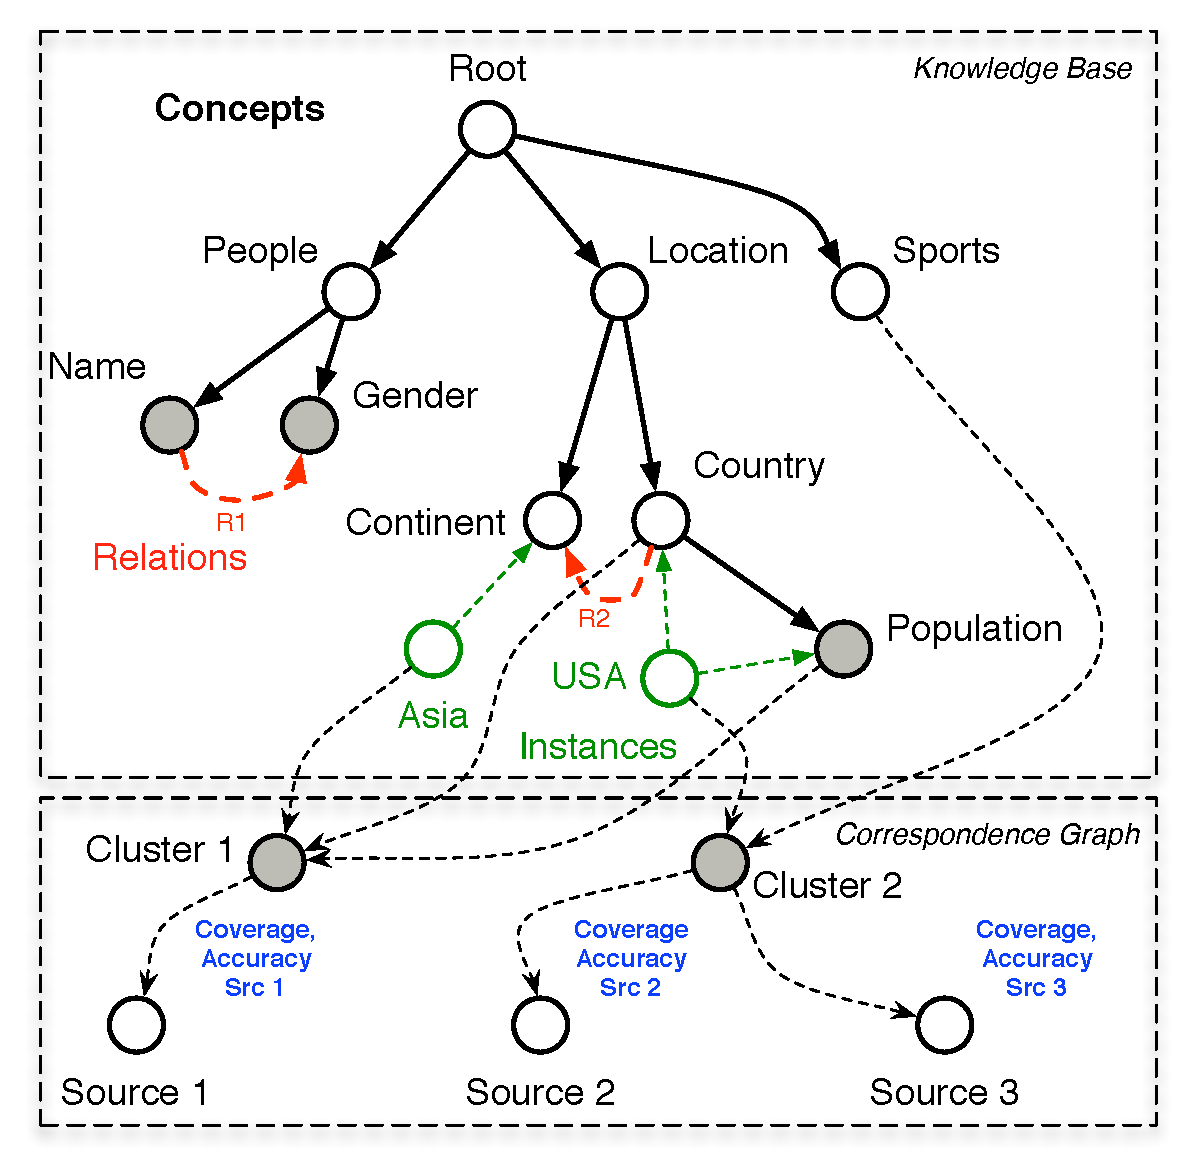
\includegraphics[clip,scale=0.36]{fig/kgcg}
	\vspace{-5pt}
	\caption{An example of a knowledge base and a correspondence graph with two cluster nodes corresponding to the population of countries in Asia and sports in the USA.}
	\label{fig:kgcg}
	\end{center}
	\vspace{-20pt}
\end{figure}
Specifically, the nodes in the correspondence graph are either data sources (referred to as {\em source nodes}) or clusters of concepts and/or entities as dictated by the available sources (called {\em cluster nodes}). The edges in the correspondence graph connect each source node with cluster nodes and cluster nodes with the corresponding concepts and entities in the knowledge base.  Each edge from a source to a cluster node is annotated with a quality profile of that source for that specific cluster, and each cluster node is associated with local information about the dependencies of the data sources that are connected to it. An example of a knowledge base and a correspondence graph is shown in \Cref{fig:kgcg}. There are two cluster nodes, one corresponding to the population of countries in Asia and one to sports in the USA. 

We describe a preliminary approach for constructing the correspondence graph. We propose a two step approach where we first learn the latent cluster nodes and then compute the quality profiles and data source dependencies for each cluster node. 

\vspace{3pt} \noindent\textbf{Step 1.} The cluster nodes in the correspondence graph can be viewed as a content-based clustering of the available data sources. Furthermore, each of these nodes is associated with a collection of concepts and/or instances of the knowledge base. The following approach can be used to construct these nodes. Each source can be viewed as a {\em collection of entries}, where each entry is a {\em conjunction} over concepts and/or instances. To obtain this representation, we must annotate the content of each source with concept and instance labels from the knowledge graph. Several techniques have been proposed for obtaining these annotations~\cite{spotlight,limaye:2010}. Once the content of sources is represented as a collection of concept and instance conjunctions, one can use a {\em mixed membership model}~\cite{blei:2003} to describe how the content of sources is generated considering the cluster nodes. Each source is modeled as a mixture over the cluster nodes. The cluster nodes are shared across all sources but the mixture proportions vary from source to source (they can also be zero). Each cluster node describes a distribution over concepts or events. We plan on building upon recent work on sparsity inducing non-parametric latent variable learning techniques~\cite{elidan:2005, sdm:2013}. Sparsity is necessary as each cluster node should contain only a limited number of concepts and instances. 

\vspace{3pt} \noindent\textbf{Step 2.} After discovering the cluster nodes, we can compute the quality of each source with respect to each cluster node it is connected to. To do the latter, we need to collectively analyze the content of all sources connected to a cluster node. We propose following an approach similar to Rekatsinas et al.~\cite{rekatsinas:2014} where samples from all the sources are integrated into a single dataset forming the content of the cluster and then each individual sample is compared with the integrated data to compute the source quality. 

Apart from the individual source quality profiles, we also need to learn the quality dependencies across sources. Recall that the quality metrics presented in \Cref{sec:quality} 
can be expressed as probability distributions. When sources are dependent, the random variables corresponding to their quality distributions are dependent. These dependencies can be extracted from the available source samples.  We conjecture that these dependencies can be represented using a {\em factor graph}~\cite{koller:2009}, i.e., a particular type of graphical model that enables efficient computation of marginal distributions, over the source random variables. We plan to explore how structure learning techniques from the statistical relational learning literature~\cite{getoor:2007} can be used to solve this problem. These factor graphs will also enable computing the quality of an arbitrary set of sources via probabilistic inference. The latter is necessary for solving the problem of sources selection during query time as we describe next. 

\subsection{Query Engine}
\label{sec:queryengine}
Queries in the context of a data source management system correspond to descriptions of the user's integration requirements. We envision a system where queries are free-text descriptions containing references to multiple entities and concepts. Part of the query will correspond to specifying an integration budget constraint either in terms of the maximum amount of money to spend for acquiring data or the maximum number of sources to be used for the task. Finally, the user will have the capability of selecting which quality metrics are relevant to her integration task. Given the user requirements as input the query engine should perform the following steps: (i) analyze the description of the integration task and reason about its semantic content by mapping concept or entity mentions to the knowledge base, (ii) identify the relevant cluster nodes in the correspondence graph and retrieve the sources that are relevant to the user's input, (iii) find Pareto optimal source selection solution considering the quality and cost specifications of the user, (iv) present these solutions to the user and allow the interactive exploration of the retrieved results.

\vspace{3pt}\noindent\textbf{Semantic Analysis.} The concepts or entities mentioned in the query can vary significantly. Queries can also be ambiguous (e.g., Apple the company versus apple the fruit). To handle such cases a data source management system should be able to reason about the semantic content of user descriptions. Techniques from keyword search over knowledge bases applied to lists~\cite{pimplikar:2012} or web-tables~\cite{dassarma:2012} can be extended to support these needs. Once the query concepts and entities are retrieved, the query engine needs to identify the relevant cluster nodes. Following the mixed membership model described above, we can consider the query as a collection of concepts and instances and find its mixture proportions with respect to the cluster nodes in the correspondence graph. Inferring the mixture proportions can be done using approaches similar to the ones introduce by Blei et al.~\cite{blei:2003}. Once the mixture proportions are known, we can identify the sources that are relevant to each of the cluster nodes having a non-zero mixture proportion for the query by traversing the correspondence graph. To identify the set of valuable sources for the given query we can solve the problem of source selection~\cite{dong:vldb13, rekatsinas:2014}. The benefit of integration can be described as a linear combination of the integration quality of each individual cluster node using the mixture proportions as weights.
\begin{figure}
	\begin{center}
	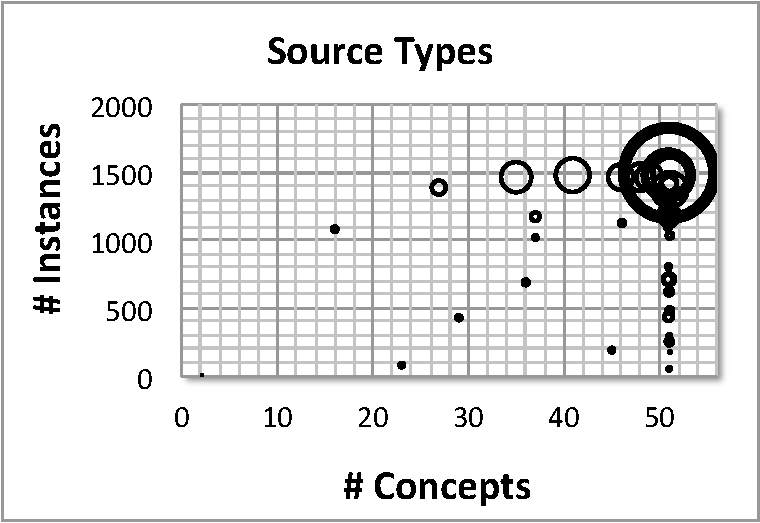
\includegraphics[clip,scale=0.36]{fig/sources.pdf}
	\vspace{-5pt}
	\caption{An illustrative bubble chart describing the sources of a potential solution to a user query.}
	\label{fig:bubble}
	\end{center}
	\vspace{-25pt}
\end{figure}

\vspace{3pt}\noindent\textbf{Pareto Optimal Answers.} Source selection identifies the optimal set of sources to be used for a specific integration task by trying to maximize the profit of integration with respect to any budget constraints. As mentioned in the previous section, source selection should be cast as a multi-objective optimization problem and the query engine should be able to find the set of Pareto optimal solutions. Discovering all the solutions on the Pareto front might be expensive, thus, efficient approximation and exploration techniques have been proposed in the optimization literature~\cite{wilson:2001}. Moreover, algorithms for computing the Pareto frontier of a finite set of alternatives have been studied in the skyline query literature~\cite{godfrey:2007,kossmann:2002}. 

\vspace{3pt}\noindent\textbf{Interactive Exploration.} We propose a two-level visualization approach for exploring solutions on the Pareto front.  We argue that the query engine system should return a ranked list with {\em diverse} solutions on the Pareto frontier and mention the quality characteristics for the selected set of sources, the number of sources and the total integration cost. If the user selects to explore the content of the solution the system will present a bubble chart with all the sources in the solution. The dimensions of the bubble chart should characterize the content of each source while the size of the bubble should correspond to the actual size (with respect to number of entries) of each source. We argue that the following dimensions are necessary to describe each source: (i) the {\em concept focus} of the source, i.e., number of different concepts mentioned in the source, and (ii) the {\em instance focus} of the source, i.e., the number of different instances mentioned in the source. If the user selects a specific bubble from the bubble chart, details regarding the name and quality of the sources should be presented to the user. This information can be directly retrieved from the correspondence graph and does not need to be computed during query time. An example of such a bubble chart is shown in \Cref{fig:bubble}. Finally, we envision a system that will provide the user with the capability of exploring the neighborhood of a solution from the initial list. This can be done either (i) by removing sources from a running solution or (ii) by recommending solutions in the Pareto frontier neighborhood of the running solution. These functionalities require reasoning about the distance of solutions on the Pareto frontier introducing a new challenge.


\section{Related Work}
\label{sec:related}
Prior work mainly focuses on isolated aspects of data source management, and to our knowledge, there has been no systematic approach to developing a source management system over large numbers of data sources. There is much work on schema mapping and semantic integration of different
sources~\cite{cafarella:2009,venetis:11, oktie:13}. This line of work focuses on the construction of a global schema or a knowledge base describing the domain of the data sources, and its final goal is not reasoning about the content and quality of sources. Moreover, most of that work focuses on sources from a specific domain and does not present results for largely heterogeneous sources. Web table search~\cite{cafarella:2009,limaye:2010, dassarma:2012,yakout:2012, fan:2014} is also closely related to data source search. Most of the proposed techniques consider user queries and return tables related to specific keywords present in the query. However, the keyword-based techniques fail to capture the semantics of natural language, i.e., the intentions of the users, and thus they can only go as far as giving relevant hits. Using the knowledge base as the entry point of data source search will enable us to clearly capture the intentions of the user and return more useful results. Further, extending data source search to recommend sets of sources to be integrated and analyzed collectively, as we propose to do, is a useful functionality in many domains (e.g., data driven journalism) where users are not experts and want an efficient way of exploring multiple data sources. \textcolor{red}{Apart from Web table search, more generic data search systems, such as Microsoft Power BI~\cite{powerbi} have been recently proposed. Nevertheless, such systems focus on facilitating the integration of diverse data sources and do not provide analysts with the functionality to understand the quality of data sources and the trade-off between different quality metrics.} Finally, our work on source selection~\cite{dong:vldb13, rekatsinas:2014} has considered problems where all sources follow a common schema and focus on a single data domain.

\section{Conclusions}
\label{sec:conclusion}
In this paper, we argued that due to the vast numbers of available data sources, it is not beneficial for users to integrate all available sources as this can be either detrimental to the quality for the integration result or very expensive due to the fees sources charge to grant access to their data. We presented our vision for a data source management system that will enable users to discover the most valuable sources for their applications. Given a user's budget our system also enables the interactive exploration of different sets of sources allowing the user to truly understand the quality and cost trade-off between different integration options. We discussed the major challenges in building such a system such as, supporting diverse integration tasks and multiple users, assessing the quality of data sources and enabling the interactive exploration over different sets of sources. We presented a preliminary design of such a system addressing these challenges. We believe that it is the time for a new type of data portals that will allow data scientists and analysts to find the most valuable data sets for their tasks and limit the person-hours spent in validating the quality of data. 

\subsection*{Acknowledgements}\vspace{-5pt}
The authors would like to deeply thank Amol Deshpande for the many fruitful and insightful discussions on the subject as well as his help on 
proofreading the manuscript. This paper would not have been possible without his help. 

This work is supported by the Intelligence Advanced Research Projects Activity (IARPA) via Department of Interior National Business Center (DoI/NBC) contract number D12PC000337, the US Government is authorized to reproduce and distribute reprints for Governmental purposes notwithstanding any copyright annotation thereon. Disclaimer: The views and conclusions contained herein are those of the authors and should
not be interpreted as necessarily representing the official policies or endorsements, either expressed or implied, of IARPA, DoI/NBC, or the
US Government.


\begin{thebibliography}{10}

\bibitem{spotlight}
Dbpedia spotlight.
\newblock \url{https://github.com/dbpedia-spotlight/}.

\bibitem{powerbi}
Excel Power BI.
\newblock \url{http://www.microsoft.com/en-us/powerbi}.

\bibitem{sdm:2013}
R.~Balasubramanyan and W.~W. Cohen.
\newblock Regularization of latent variable models to obtain sparsity.
\newblock In {\em SDM}, 2013.

\bibitem{balazinska:vldb11}
M.~Balazinska, B.~Howe, and D.~Suciu.
\newblock Data markets in the cloud: An opportunity for the database community.
\newblock {\em PVLDB}, 4, 2011.

\bibitem{berti-equille:sailing}
L.~Berti-Equille, A.~D. Sarma, X.~Dong, A.~Marian, and D.~Srivastava.
\newblock Sailing the information ocean with awareness of currents: Discovery
  and application of source dependence.
\newblock In {\em CIDR}, 2009.

\bibitem{blei:2003}
D.~M. Blei, A.~Y. Ng, and M.~I. Jordan.
\newblock Latent dirichlet allocation.
\newblock {\em J. Mach. Learn. Res.}, Mar. 2003.

\bibitem{bronzi:2013}
M.~Bronzi, V.~Crescenzi, P.~Merialdo, and P.~Papotti.
\newblock Extraction and integration of partially overlapping web sources.
\newblock {\em PVLDB}, 3, 2013.

\bibitem{cafarella:2009}
M.~J. Cafarella, A.~Halevy, and N.~Khoussainova.
\newblock Data integration for the relational web.
\newblock {\em PVLDB}, 2009.

\bibitem{dassarma:2012}
A.~Das~Sarma, L.~Fang, N.~Gupta, A.~Halevy, H.~Lee, F.~Wu, R.~Xin, and C.~Yu.
\newblock Finding related tables.
\newblock {\em SIGMOD}, 2012.

\bibitem{dong:2009}
X.~L. Dong, L.~Berti-Equille, and D.~Srivastava.
\newblock Integrating conflicting data: The role of source dependence.
\newblock {\em PVLDB}, 2, 2009.

\bibitem{Dong_vldb:2009}
X.~L. Dong, A.~Halevy, and C.~Yu.
\newblock Data integration with uncertainty.
\newblock {\em The VLDB Journal}, Apr. 2009.

\bibitem{dong:vldb13}
X.~L. Dong, B.~Saha, and D.~Srivastava.
\newblock Less is more: selecting sources wisely for integration.
\newblock {\em PVLDB}, 2013.

\bibitem{elidan:2005}
G.~Elidan and N.~Friedman.
\newblock {Learning Hidden Variable Networks: The Information Bottleneck
  Approach}.
\newblock {\em J. Mach. Learn. Res.}, 2005.

\bibitem{fan:2014}
J.~Fan, M.~Lu, B.~C. Ooi, W.-C. Tan, and M.~Zhang.
\newblock A hybrid machine-crowdsourcing system for matching web tables.
\newblock In {\em ICDE}, 2014.

\bibitem{getoor:2007}
L.~Getoor and B.~Taskar.
\newblock {\em {Probabilistic Relational Models}}.
\newblock The MIT Press, 2007.

\bibitem{godfrey:2007}
P.~Godfrey, R.~Shipley, and J.~Gryz.
\newblock Algorithms and analyses for maximal vector computation.
\newblock {\em The VLDB Journal},16(1), 2007.

\bibitem{oktie:13}
O.~Hassanzadeh, K.~Q. Pu, S.~H. Yeganeh, R.~J. Miller, L.~Popa, M.~A.
  Hern{\'a}ndez, and H.~Ho.
\newblock Discovering linkage points over web data.
\newblock {\em PVLDB}, 6, 2013.

%\bibitem{oktie:11}
%O.~Hassanzadeh, S.~H. Yeganeh, and R.~J. Miller.
%\newblock Linking semistructured data on the web.
%\newblock In {\em WebDB}, 2011.

\bibitem{koller:2009}
D.~Koller and N.~Friedman.
\newblock {\em Probabilistic Graphical Models: Principles and Techniques -
  Adaptive Computation and Machine Learning}.
\newblock The MIT Press, 2009.

\bibitem{kossmann:2002}
D.~Kossmann, F.~Ramsak, and S.~Rost.
\newblock Shooting stars in the sky: An online algorithm for skyline queries.
\newblock {\em VLDB}, 2002.

\bibitem{li:2012}
X.~Li, X.~L. Dong, K.~Lyons, W.~Meng, and D.~Srivastava.
\newblock Truth finding on the deep web: is the problem solved?
\newblock {\em VLDB}, 2013.

\bibitem{limaye:2010}
G.~Limaye, S.~Sarawagi, and S.~Chakrabarti.
\newblock Annotating and searching web tables using entities, types and
  relationships.
\newblock {\em PVLDB}, 3, 2010.

\bibitem{pang:2002}
B.~Pang, L.~Lee, and S.~Vaithyanathan.
\newblock Thumbs Up?: Sentiment Classification Using Machine Learning Techniques.
\newblock {\em ACL}, 2002.

\bibitem{pimplikar:2012}
R.~Pimplikar and S.~Sarawagi.
\newblock Answering table queries on the web using column keywords.
\newblock {\em PVLDB}, 5, 2012.

\bibitem{pipino:2002}
L.~L. Pipino, Y.~W. Lee, and R.~Y. Wang.
\newblock Data quality assessment.
\newblock {\em Commun. ACM}, 45(4), 2002.

\bibitem{pochampally:2014}
R.~Pochampally, A.~Das~Sarma, X.~L. Dong, A.~Meliou, and D.~Srivastava.
\newblock Fusing data with correlations.
\newblock {\em SIGMOD}, 2014.

\bibitem{rekatsinas:2014}
T.~Rekatsinas, X.~L. Dong, and D.~Srivastava.
\newblock Characterizing and selecting fresh data sources.
\newblock {\em SIGMOD}, 2014.

\bibitem{schutte:2014}
S.~Schutte and K.~Donnay.
\newblock Matched wake analysis: finding causal relationships in spatiotemporal
  event data.
\newblock {\em Political Geography}, 41, 2014.

\bibitem{kg}
A.~Singhal.
\newblock Introducing the knowledge graph: Things, not strings.
\newblock Official Blof (of Google), 2012.

\bibitem{venetis:11}
P.~Venetis, A.~Y. Halevy, J.~Madhavan, M.~Pasca, W.~Shen, F.~Wu, G.~Miao, and
  C.~Wu.
\newblock Recovering semantics of tables on the web.
\newblock {\em PVLDB}, 4, 2011.

\bibitem{wilson:2001}
B.~Wilson, D.~Cappelleri, T.~W. Simpson, and M.~Frecker.
\newblock {Efficient Pareto Frontier Exploration using Surrogate
  Approximations}.
\newblock {\em Optimization and Engineering}, 2, 2001.

\bibitem{yakout:2012}
M.~Yakout, K.~Ganjam, K.~Chakrabarti, and S.~Chaudhuri.
\newblock Infogather: entity augmentation and attribute discovery by holistic
  matching with web tables.
\newblock {\em SIGMOD}, 2012.

\end{thebibliography}

\appendix
%Appendix A
\section{Demo Proposal}
Here, we describe a demo proposal for the data source management prototype introduced in \Cref{sec:corgraph}. The main focus of the data source management system introduced before is to enable users to discover and explore valuable sets of sources for diverse integration tasks. In this way, the demo focuses on exposing these functionalities to the audience. 

\vspace{3pt}\noindent\textbf{Set-up and Scenarios.} The main idea for the demo is that the audience will get direct access to a prototype of our source management system. We will provide access to our system via a web-interface for this purpose. The data and the system will be stored and running on a remote server, however, the audience will have the opportunity to explore the internal source indexing mechanism of our system and issue source selection queries against it. 

For the purpose of the demonstration we will focus on data extracted from the Global Database of Events, Languages and Tone (GDELT)~\cite{leetaru_ap:2013}. GDELT is a repository that monitors news media from all over the world and extracts georeferenced records that correspond to different events and interactions between diverse groups of people, international organizations, countries etc. GDELT gets updated every day with new event extractions. This repository is rather prominent amongst political scientists and data mining scientists as they use it to find supporting evidence for new theories~\cite{schutte_ap:2014} and validate new techniques for forecasting events of interest~\cite{keneshloo_ap:2014} (e.g., civil unrest events). 

We believe that GDELT is the right fit to demonstrate the usefulness and practicality of our data source management system due to the large number of data sources available, the available daily updates and the heterogeneity that sources exhibit both with respect to their content and their quality. In our recent work on source selection~\cite{rekatsinas_ap:2014}, we studied a snapshot of GDELT over a period of one month from January 2014 to February 2014 and have evaluated the effectiveness of source selection. That snapshot contained 15,275 news sources providing 2,219,704 distinct events corresponding to 242 different locations and 236 different event concepts. We refer the reader to Rekatsinas et al.~\cite{rekatsinas_ap:2014} for a more detailed description of the data set. For this demo we plan to use a recent larger snapshot of GDELT including all sources contained in the dataset. We aim to enable daily updates in our data source management system.

\vspace{3pt}\noindent\textbf{Correspondence Graph Exploration.} During the first part of the demonstration, users will be able to explore the correspondence graph part of our system. In particular, we will provide visualizations illustrating a fixed set of source nodes together with their corresponding cluster nodes and quality summaries. Moreover, the users will have the capability of selecting a specific cluster node and see the different concepts and entities connected with it.

\vspace{3pt}\noindent\textbf{Source Selection Queries.} For the second part of the demonstration, we will provide the users with a set of example queries they can execute against our system. The users will have the opportunity to explore the solutions for these queries using the techniques introduced in \Cref{sec:queryengine}. Our goal is for users to understand the trade-offs between different quality metrics (including coverage, timeliness and accuracy) of sources in GDELT. Users will also have the opportunity to issue their own free-text queries.

\vspace{3pt}\noindent\textbf{Summary.} Overall, the demo will allow users to: (i) understand the internal source indexing mechanism (i.e., the correspondence graph) of our prototype system, (ii) issue queries against it and (iii) explore the corresponding source selection solutions via a web-interface. Users will need to play the role of a political scientist and use our system to discover the most valuable sources for their own analysis applications.
 \balance

\begin{thebibliography}{10}

\bibitem{keneshloo_ap:2014}
Y.~Keneshloo, J.~Cadena, G.~Korkmaz, and N.~Ramakrishnan.
\newblock Detecting and Forecasting Domestic Political Crises: A Graph-based Approach.
\newblock {\em WebSci}, 2014.

\bibitem{leetaru_ap:2013}
K.~Leetaru and P.~Schrodt.
\newblock Gdelt: Global data on events, language, and tone, 1979-2012.
\newblock {\em Inter. Studies Association Annual Conf.}, 2013.

\bibitem{rekatsinas_ap:2014}
T.~Rekatsinas, X.~L. Dong, and D.~Srivastava.
\newblock Characterizing and selecting fresh data sources.
\newblock {\em SIGMOD}, 2014.

\bibitem{schutte_ap:2014}
S.~Schutte and K.~Donnay.
\newblock Matched wake analysis: finding causal relationships in spatiotemporal
  event data.
\newblock {\em Political Geography}, 41, 2014.


\end{thebibliography}

\end{document}
